\chapter{Profilo dei cigli}

Un altro grafico elaborato dal programma mostra come variano i valori di sopraelevazione, ovvero delle pendenze trasversali. Per creare una sopraelevazione, si sfrutta un template già preimpostato per categoria di strada: esso deve rispettare la tipologia di strada F extraurbana (\ref{template}), per cui dal decreto ministeriale del 5/11/2001 si leggono i valori di larghezza minima della corsia e della banchina.

\begin{figure}[H]
    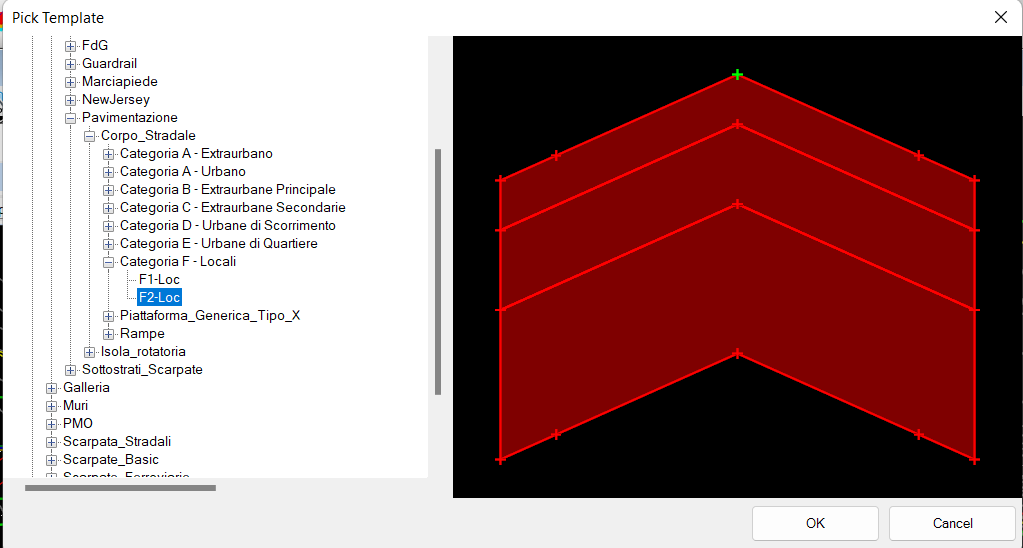
\includegraphics[width=\textwidth]{Figures/template.png}
      \caption{template f1-loc}
      \label{template}
\end{figure}

Utilizzando il comando Create Superelevation Section nella sezione Corridors/Superelevation si creerà la sopraelevazione (\ref{Sopraelevazione}) che sarà visibile sul tracciato planimetrico.

\begin{figure}[H]
    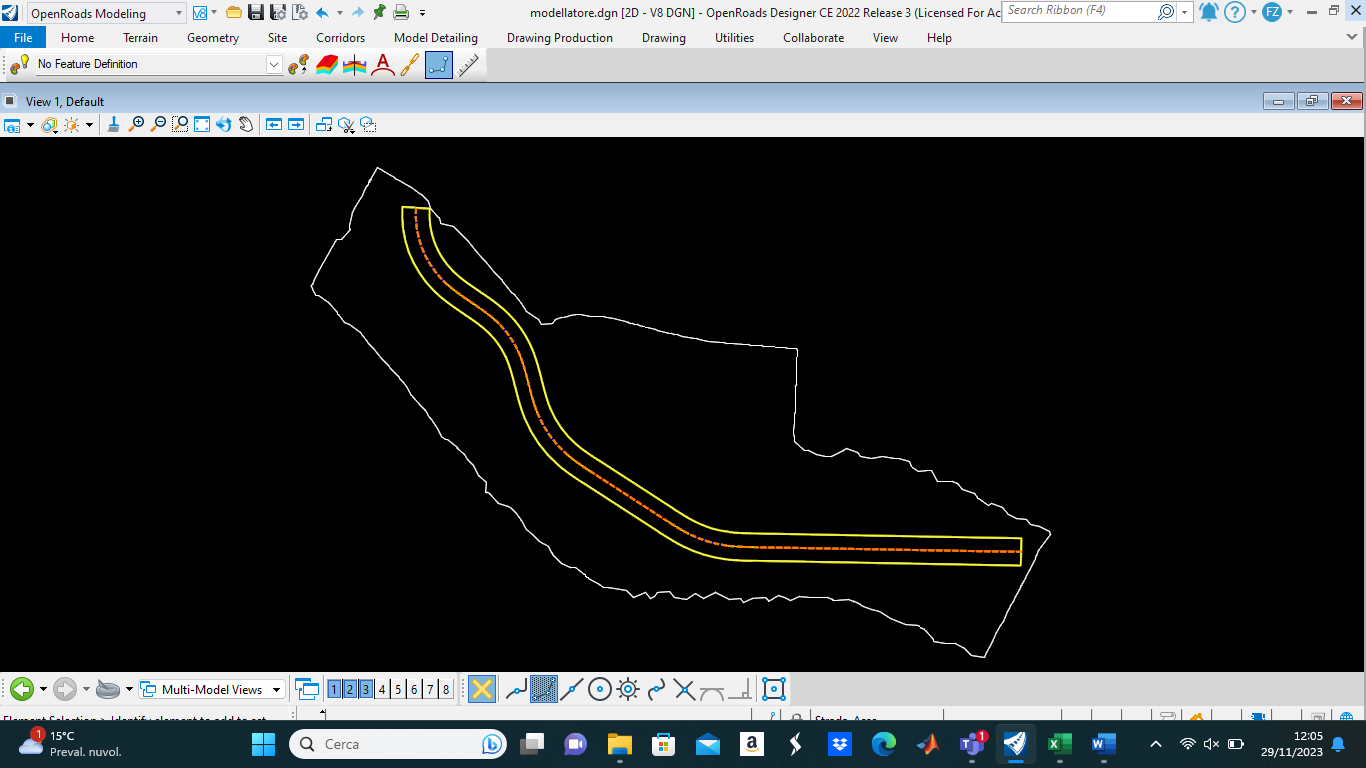
\includegraphics[width=\textwidth]{Figures/Sopraelevazione del tracciato vista in pianta.png}
      \caption{Sopraelevazione del tracciato vista in pianta}
      \label{Sopraelevazione}
\end{figure}

Utilizzando ora il comando Calculate Superelevation il programma produrrà il profilo dei cigli (\ref{Profilo dei cigli}) del nostro tracciato.

\begin{figure}[H]
    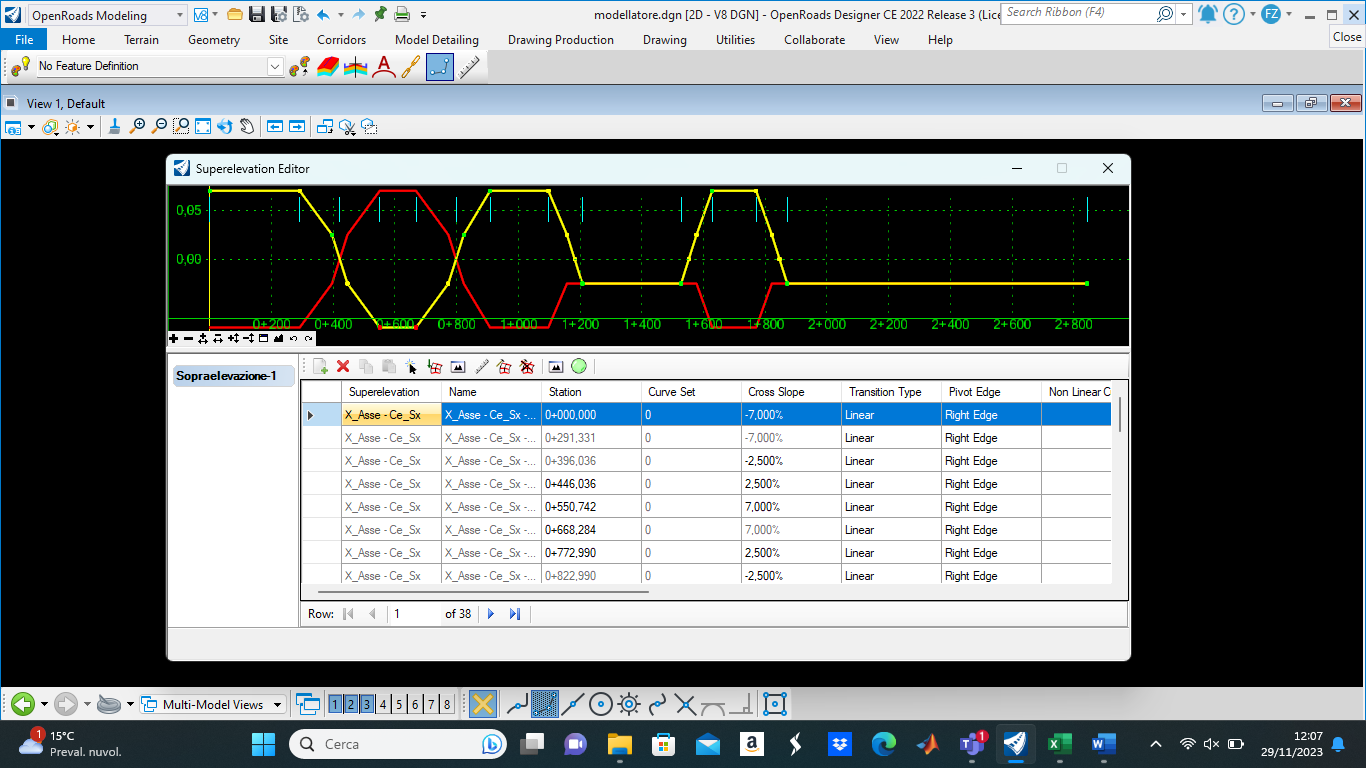
\includegraphics[width=\textwidth]{Figures/Profilo dei cigli.png}
      \caption{Profilo dei cigli}
      \label{Profilo dei cigli}
\end{figure}

